\documentclass[a4paper]{article}
\usepackage[margin=1in]{geometry}%设置边距,符合Word设定
\usepackage{amssymb,amsfonts,amsmath,amsthm}
\usepackage{ctex}
\usepackage{setspace}
\usepackage{lipsum}
\usepackage{graphicx}%插入图片
\graphicspath{{Figures/}}%文章所用图片在当前目录下的 Figures目录

\usepackage{hyperref} % 对目录生成链接,注:该宏包可能与其他宏包冲突,故放在所有引用的宏包之后
\hypersetup{colorlinks = true,  % 将链接文字带颜色
	bookmarksopen = true, % 展开书签
	bookmarksnumbered = true, % 书签带章节编号
	pdftitle = 第二章扩展作业, % 标题
	pdfauthor = 刘正浩 2019270103005} % 作者

%\renewcommand{\contentsname}{\centerline{Contents}} %经过设置word格式后,将目录标题居中


\title{\heiti\zihao{2} 第二章扩展作业}
\author{\songti 刘正浩 2019270103005}
\date{2021.4.18}


\begin{document}
	\maketitle
	\thispagestyle{empty}

	%\begin{abstract}
	%	\lipsum[2]
	%\end{abstract}

	\tableofcontents

	\section{证明线电荷守恒定律}
		证明微观表达式与宏观表达式等价。
		
		设有一段曲线上分布着线密度为$\sigma$的电荷,起点和终点的坐标分别为a和b,如图1。
		\begin{figure}[htbp]
			\centering
			
\includegraphics[scale=0.8]{1.png}
			\caption{曲线的形状(直径应为0,图中为表现清楚而夸大了直径。)}
		\end{figure}

		根据线电荷守恒定律的宏观表达式
		\begin{equation}
			i_{a} - i_{b} = \frac {\mathrm{d}q} {\mathrm{d}t}
		\end{equation}
		可以得到
		\begin{equation}
			\mathrm{d}q = (i_{a}-i_{b}) \mathrm{d}t
		\end{equation}

		另一方面,由线电荷密度可以知道,这一段曲线上分布的总电荷为
		\begin{equation}
			q = \int _ a ^ b \sigma \mathrm{d}l
		\end{equation}
		\begin{equation}
			\mathrm{d}q = \int _ a ^ b \mathrm{d}\sigma \mathrm{d}l
		\end{equation}

		将2、4式联立可得
		\begin{equation}
			\frac{\mathrm{d}I}{\mathrm{d}l} = - \frac{\mathrm{d}\sigma}{\mathrm{d}t}
		\end{equation}
	\section{证明两电荷作用力在连线方向}
		使用反证法证明两电荷作用力在连线方向。假设两电荷之间的作用力不在连线方向。
		\subsection{情况1}
			假设两电荷受到的力有垂直于连线方向,并且互相相反的分量,如图2所示。
			由于两个分量的力矩方向相同且不为0,所以由两个电荷组成的系统将围绕质量中心开始旋转,角动量不守恒。所以这种情况不可能发生。
			\begin{figure}[htbp]
				\centering
				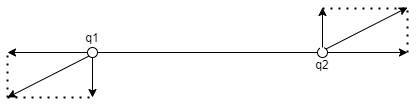
\includegraphics[scale=0.7]{2.1.png}
				\caption{两垂直分量方向相反}
			\end{figure}

		\subsection{情况2}
			仍然假设两电荷受到的力垂直于连线方向且方向相同,如图3所示。
			由于整个系统受力不平衡,所以动量不守恒,这种情况不可能发生。
			\begin{figure}[htbp]
				\centering
				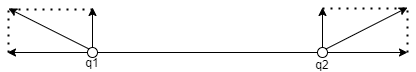
\includegraphics[scale=0.7]{2.2.png}
				\caption{两垂直分量方向相同}
			\end{figure}

		综上所述,两电荷的作用力在连线方向。

	\section{第三题}
		平面S'是一个无限大的平面,源点在球面外。设源点在平面上的投影为$P_0$。则对平面上的任意一点$P$,它对应的
		$\vec{e_R}\cdot\mathrm{d}\vec{S}$在S'平面上的分量都可以与$P$点关于$P_0$点的对称点$P'$对应的
		$\vec{e_R}\cdot\mathrm{d}\vec{S}$在S'平面上的分量相抵消。其结果是:
		\begin{equation}
			\vec{e_R}\cdot\mathrm{d}\vec{S} = \mathrm{d}S
		\end{equation}
		故
		\begin{equation}
			\int_S \frac{\vec{e_R}}{R^2} \mathrm{d}\vec{S} = \int_S \frac{\mathrm{d}S}{R^2}
		\end{equation}
		而7式的右边刚好是无限大平面S'对应的立体角,它的值为$2\pi$。故
		\begin{equation}
			\int_S \frac{\vec{e_R}}{R^2} \mathrm{d}\vec{S} = 2\pi
		\end{equation}
		得证。

	\section{第四题}
		思路:第二行的两个积分式形式与亥姆霍兹定理的结论比较像,考虑使用亥姆霍兹定理进行证明。
		使用亥姆霍兹定理解决这个问题的前提是将场分解成散度场和旋度场,并分别求解散度源和旋度源。

	\section{第五题}
		\begin{figure}[htbp]
			\centering
			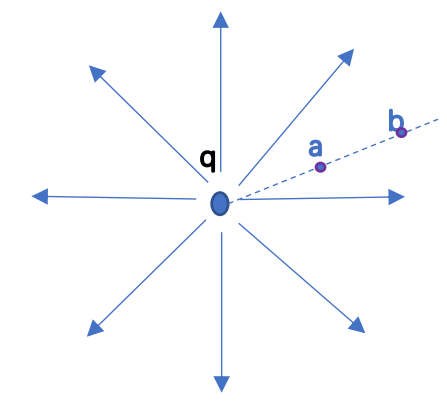
\includegraphics[scale=0.7]{5.png}
			\caption{点电荷产生的电场与a、b}
		\end{figure}
		在原式中,从$\int _{r_b} ^{r_a} \vec{E}(r)\cdot(-\vec{e_r}) \mathrm{d}l$
		到$\int _{r_b} ^{r_a} \vec{E}(r)\cdot(-\vec{e_r}) \mathrm{d}r$的一步在积分变量的替换上出现了问题。

		分析这两个积分变量可知,$\mathrm{d}l$是a与b之间的距离的微分,其值应为正数;
		而$\mathrm{d}r$是a点到源点距离与b点到源点距离的差值。在这个积分式中积分方向为从b到a,
		则这个差值的变化情况应当为从大到小,$\mathrm{d}r$应为负数。原式中将$\mathrm{d}r$当做正数来推导,自然是不对的。

		正确的推导如下:
		\begin{equation}
			\begin{split}
				V_{ba} &= \varphi(b) - \varphi(a)\\
				&= \int _{r_a} ^{r_b} \vec{E}(r)\cdot\mathrm{d}\vec{l}\\
				&= \int _{r_a} ^{r_b} \vec{E}(r)\cdot(-\vec{e_r})\mathrm{d}l\\
				&= \int _{r_a} ^{r_b} \vec{E}(r)\cdot(-\vec{e_r})(-\mathrm{d}r)\\
				&= \frac{q}{4\pi\varepsilon_0} \int _{r_a} ^{r_b} \frac{1}{r^2}\vec{e_r}\cdot\vec{e_r}\mathrm{d}r\\
				&= - \frac{q}{4\pi\varepsilon_0 r} \bigg| _{r_b} ^{r_a}\\
				&= \frac{q}{4\pi\varepsilon_0} \bigg(\frac{1}{r_b} - \frac{1}{r_a} \bigg)\\
				&= \varphi(b)-\varphi(a)
			\end{split}
		\end{equation}
	
	\section{第六题}

	\section{第七题}
		电介质球内部的极化电荷体密度为:
		\begin{equation}
			\begin{split}
				\rho_p &= - \nabla \cdot \vec{P}\\
				&= - \frac{1}{r^2} \frac{\mathrm{d}}{\mathrm{d}r}(r^2 P_r)\\
				&= - \frac{1}{r^2} \frac{\mathrm{d}}{\mathrm{d}r} \bigg( r^2 \frac{k}{r} \bigg)\\
				&= - \frac{k}{r^2}
			\end{split}
		\end{equation}
		电介质球表面的极化电荷面密度为:
		\begin{equation}
			\rho _{SP} = \vec{P} \cdot \vec{e_n} = \vec{e_r} \frac{k}{r} \cdot \vec{e_r}  \bigg | _{r=a} = \frac{k}{a}
		\end{equation}
		球内部的极化电荷量为:
		\begin{equation}
			Q_P = \int _0 ^a -\frac{k}{r^2} 4\pi r^2 \mathrm{d}r = -4\pi ak
		\end{equation}
		球表面的极化电荷量为:
		\begin{equation}
			Q_{SP} = S \cdot \rho _{SP} = 4\pi a^2 \frac{k}{r} \bigg| _{r=a} = 4\pi ak
		\end{equation}
		可以看出,球表面的极化电荷量与球内部的极化电荷量的和为零,而电介质球在极化之前也是不带电的,
		所以在极化过程中电荷守恒。

	\section{第八题}

	\section{第九题}
		思路与第四题基本一致。
	\section{第十题}
		\begin{figure}[htbp]
			\centering
			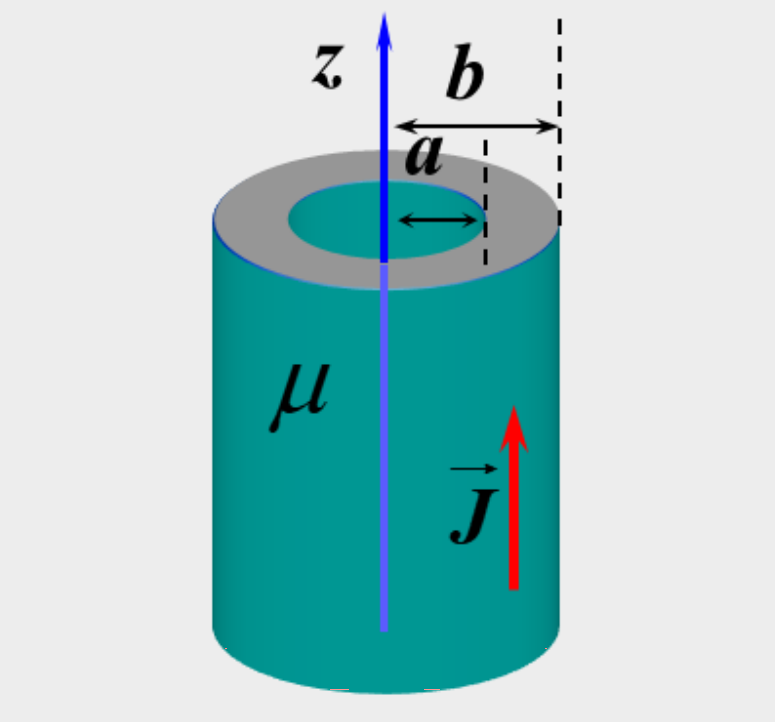
\includegraphics[scale=0.5]{10.png}
			\caption{圆筒形磁介质}
		\end{figure}
		体磁化电流密度为:
		\begin{equation}
			\vec{J_M} = \nabla \times (\chi_m \vec{H})=\chi_m \vec{J}
		\end{equation}
		面磁化电流密度为:
		\begin{equation}
			\begin{split}
				\vec{J_{SM}} &= \vec{M} \times \vec{e_n}\\
				&= \chi_m \bigg(\frac{J_0 (r^2 - a^2)}{2r} \bigg) \vec{e_\phi} \times \vec{e_n}\\
			\end{split}
		\end{equation}
		体磁化电流为:
		\begin{equation}
			I_M = \int _a ^b 2\pi r\chi_m J_0 \vec{e_z}\mathrm{d}r = (b^2 - a^2)\chi_m\pi J_0
		\end{equation}
		面磁化电流为:
		\begin{equation}
			\begin{split}
				I_{SM} &= 2\pi b|\vec{J_{SM}}| \bigg| _{r=b}\\
				&= -2\pi b \frac{J_0(b^2 - a^2)\chi_m\pi}{2\pi b}\\
				&= -(b^2 - a^2)\chi_m \pi J_0
			\end{split}
		\end{equation}
		可知体磁化电流与面磁化电流之和为0.
	\section{第十一题}
		\begin{figure}[htbp]
			\centering
			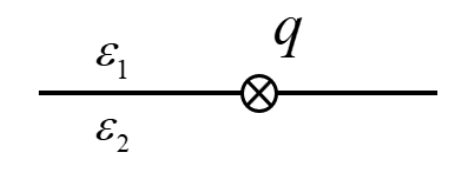
\includegraphics[scale=0.7]{11.png}
			\caption{介质与点电荷}
		\end{figure}
		由于只有静止点电荷,所以磁场强度与磁感应强度均为0。
		\begin{equation}
			\begin{split}
				\vec{e_n} \times (\vec{H_1} - \vec{H_2}) = 0\\
				\vec{e_n} \cdot (\vec{B_1} - \vec{B_2}) = 0
			\end{split}
 		\end{equation}
	\section{第十二题}
		\begin{figure}[htbp]
			\centering
			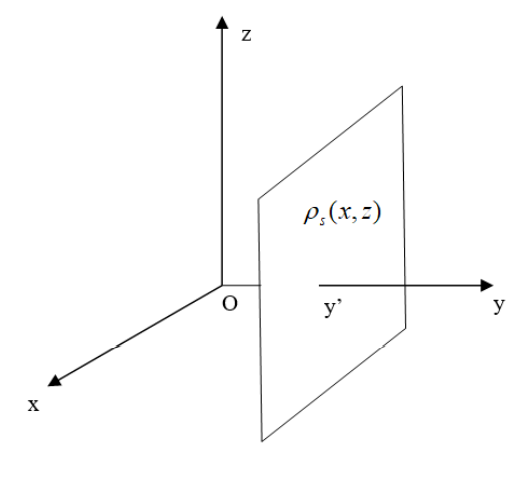
\includegraphics[scale=0.6]{12.png}
			\caption{电荷的空间分布}
		\end{figure}
		从xyz空间看,电荷只分布在坐标为$y=y'$的平面上,所以可以用冲激函数来描述这种分布情况。
		\begin{equation}
			\rho(x,y,z) = \rho_S(x,z) \cdot \delta(y-y')
		\end{equation}
	\section{第十三题}
		\begin{figure}[htbp]
			\centering
			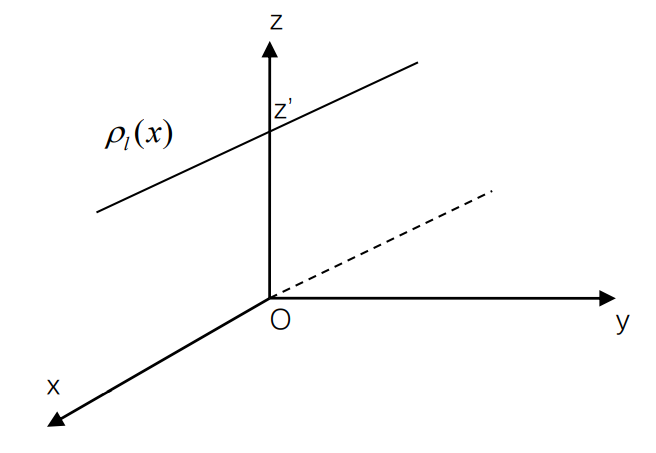
\includegraphics[scale=0.6]{13.png}
			\caption{电荷的空间分布}
		\end{figure}
		从xOz平面看,电荷只分布在坐标为$z=z'$的直线上。
		\begin{equation}
			\rho_S(x,z) = \rho_l(x) \cdot \delta(z-z')
		\end{equation}
		从xyz空间看,电荷分布在面xOz中的线$z=z'$上。
		\begin{equation}
			\begin{split}
				\rho(x,y,z) &= \rho_S(x,z) \cdot \delta(y)\\
				&= \rho_l(x) \cdot \delta(z-z') \cdot \delta(y)
			\end{split}
		\end{equation}
	\section{第十四题}
		\begin{figure}[htbp]
			\centering
			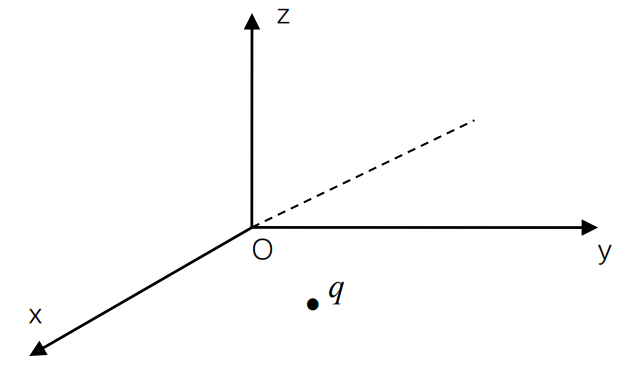
\includegraphics[scale=0.6]{14.png}
			\caption{电荷的空间分布}			
		\end{figure}
		设点电荷$q$的电荷量为$q_0$。
		\subsection{(a)}
			在xyz空间中,电荷只分布在点$(5,3,0)$处。
			\begin{equation}
				\rho(x,y,z) = q_0 \cdot \delta(x-5) \cdot \delta(y-3) \cdot \delta(z)
			\end{equation}
		\subsection{(b)}
			在xOy平面上,电荷只分布在点$(5,3)$处。
			\begin{equation}
				\rho_S(x,y) = q_0 \cdot \delta(x-5) \cdot \delta(y-3)
			\end{equation}
		\subsection{(c)}
			在穿出此点并垂直于面xOy平面的直线上,电荷只分布在$z=0$处。
			\begin{equation}
				\rho_l(z) = q_0 \cdot \delta(z)
			\end{equation}

\end{document}